\chapter{Reinforcement Learning}
\section{Motivation}
In the last chapter, we discussed the \textit{Markov Decision Process (MDP)}: a framework that models a learner's environment as a vector of states, actions, rewards, and transition probabilities. Given this model, we can solve for an optimal (reward-maximizing) policy using either value iteration or policy iteration. Sometimes, however, the learner doesn't have prior knowledge of the rewards they will get from each state or the probability distribution over states they could end up in after taking some action from their current state. Is it still possible to learn a policy that will maximize rewards? In this chapter, we will learn about \textbf{Reinforcement Learning (RL)} - a machine learning technique that addresses this problem.
\begin{mlcube}{Reinforcement Learning}
\begin{center}
    \begin{tabular}{c|c|c}
    \textit{\textbf{Domain}} & \textit{\textbf{Training}} & \textit{\textbf{Probabilistic}} \\
    \hline
    Discrete or Continuous & ? & Yes \\
    \end{tabular}
\end{center}
Note that we will only cover RL for discrete state spaces in this chapter. The question mark under the ``training" category means that RL is neither supervised nor unsupervised. 
\end{mlcube}
\section{General Approaches to RL}
Imagine that you are vacationing in a town that has 20 restaurants. Suppose that \textit{if} you had been able to try the food at every restaurant you would have had a definitive ranking of which was your favorite, second favorite, third favorite and so on. Your vacation is 10 days long and your budget allows you to eat at one restaurant per day. Your goal on your vacation is to have the best experience, which in this case means to eat at the restaurants you like the most. The problem is that you don't have enough time to figure out which restaurants you like the most since you don't have enough time to eat at each one. In this situation, you have two key considerations to balance:
\begin{enumerate}
    \item Time spent \textbf{exploring}. If you spend the right amount of time exploring new restaurants, then there is a good chance that you will find one that you like a lot. However, spending too much time exploring will result in an average experience overall since some restaurants will be good and some will be bad.
    \item Time spent \textbf{exploiting}. If you spend the right amount of time exploiting your knowledge of what restaurants you've liked the most from your exploration you will have a good experience. However, if you spend too long exploiting (and consequently less time exploring) you risk missing out on eating at all the restaurants that you could have liked \textit{more}.
\end{enumerate}
This is called the \textbf{exploration vs exploitation} tradeoff. The more time you spend exploring the less time you can spend exploiting, and vice versa. In order to have the best vacation experience, you need to find a balance between time spent exploring different restaurants and time spent exploiting what you have learned by eating at that restaurants that you liked the most thus far. A reinforcement learner's task is similar to the vacation restaurant task described above. They must balance time spent exploring the environment by taking actions and observing rewards and penalties, and time spent maximizing rewards based on what they know.\\

We now return to the problem described in the previous section: how do we learn a policy that will maximize rewards in an MDP where we know nothing about which rewards we will get from each state and which state we will end up in after taking an action? One approach is to try and \textit{learn} the MDP. In other words, we can create a learner that will explore its environment for some amount of time in order to learn the rewards associated with each state and the transition probabilities associated with each action. Then, they can use an MDP planning algorithm like policy iteration or value iteration to come up with an optimal policy and maximize their rewards. This is called \textbf{model-based} learning. The main advantage of model-based learning is that it can inexpensively incorporate changes in the reward structure or transition function of the environment into the model. However, model-based learning is computationally expensive, and an incorrect model can yield a sub-optimal policy.\\

Conversely, \textbf{model-free} learning is a family of RL techniques where a learner tries to learn the optimal policy directly without modelling the environment. While this sort of learning is less adaptive to changes in the environment, it is far more computationally efficient than model-based learning.\\

\section{Model-Free Learning}
While there are many methods within the family of model-free learning, we will focus on three \textbf{value-based} methods - \textit{SARSA} (section 12.3.1), \textit{Q-learning} (section 12.3.1) and \textit{Deep Q-learning} (section 12.3.2) - and one \textbf{policy-based} method - \textit{Policy Learning} (section 12.3.3). \\

\noindent We will begin by discussing value-based methods. In this family of RL algorithms, the learner tries to calculate the expected reward they will receive from a state $s$ upon taking action $a$. Formally, they are trying to learn a function that maps $(s, a)$ to some value representing the expected reward. This is called the Q-function and is defined as follows for some policy $\pi$:
\begin{equation}
    Q^{\pi}(s, a) = r(s, a) + \gamma\sum_{s'}p(s'|s, a)V^{\pi}(s')
\end{equation}
In words, the approximate expected reward (Q value) for taking action $s$ from state $a$ is the actual reward received from the environment by doing so in the current iteration plus the expectation taken over all reachable states of the highest value achievable starting at that state times the discount factor $\gamma$. The Q-function following the optimal policy is defined analogously:
\begin{equation}
    Q^{*}(s, a) = r(s, a) + \gamma\sum_{s'}p(s'|s, a)V^{*}(s')
\end{equation}
Note, that $V^*(s') = max_{a'}Q^*(s', a')$ since the highest value achievable from state $s'$ following policy $*$ is the Q value of taking the optimal action from $s'$. Substituting this in, we get the following \textit{Bellman Equation}:
\begin{equation}
    Q^*(s, a) = r(s, a) + \gamma\sum_s'p(s'|s, a)\max_{a'}Q^*(s', a)
\end{equation}
Note that we can't directly calculate the term $\gamma\sum_s'p(s'|s, a)\max_a'Q^*(s', a)$ since we don't know $p(s'|s, a)$. We will discuss how this is addressed by the two algorithms we will cover in the value-based family.
\subsection{SARSA and Q-Learning}
At a high level value-based model-free reinforcement learners work by initializing the values of $Q(s, a)$ for all states $s$ and all actions $a$ in an $s$ x $a$ matrix. They then repeat the following two steps until satisfactory performance is achieved: 
\begin{enumerate}
    \item \textit{Act} based on Q values
    \item Use $s$ (current state), $a$ (action), $r$ (reward), $s'$ (next state), $a'$ (action taken from next state) in order to \textit{update} the approximation of $Q(s, a)$
\end{enumerate} 
We will refer to $(s, a, r, s', a')$ as an \textbf{experience}. Let $\pi(s)$ we the action that a learner takes from state $s$. One strategy for acting that attempts to balance exploration and exploitation is called $\epsilon$\textbf{-greedy} and defined as follows:
\begin{equation}
    \pi(s) = 
    \begin{cases} 
      \arg\!\max_aQ(s, a) \text{ with probability 1 - }\epsilon \\
      \text{random with probability }\epsilon
    \end{cases}
\end{equation}
Here, $\epsilon$ is some number $\in [0, 1]$ which controls how likely the learner is to choose a random action as opposed to the currently known optimal action. Varying the value of $\epsilon$ changes the balance between exploration and exploitation.\\
Once the learner has had an experience, they can begin to learn $Q^*$. 
\begin{figure}[ht!]
    \centering
    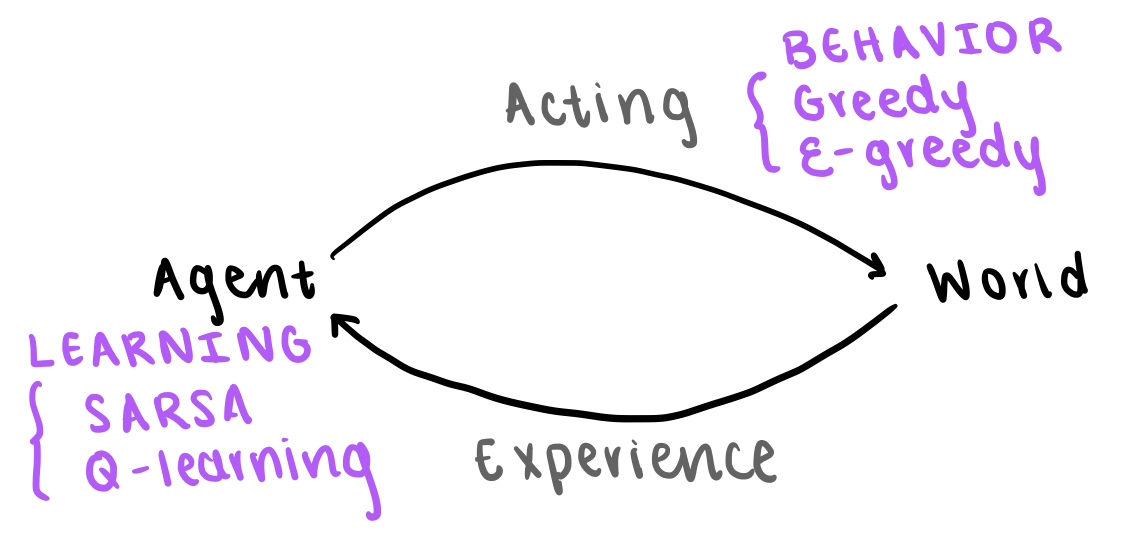
\includegraphics[scale=0.2]{../ReinforcementLearning/fig/model-free.jpeg}
    \caption{The process of model-free learning}
\end{figure}
We will now describe two algorithms which perform this update differently for every new experience:
\begin{enumerate}
    \item \textbf{SARSA}: $Q(s, a) \leftarrow \alpha_t(s, a)[r + \gamma Q(s', a') - Q(s, a)]$ where $\alpha_t(s, a)$ is the \textbf{learning rate}, a parameter which controls how much the observation affects $Q(s, a)$.\\
    The expression $r + \gamma Q(s', a')$ is a 1-step estimate of $Q(s, a)$. The expression in the square brackets above is called the \textbf{temporal difference (TD) error} and represents the difference between the previous estimate of $Q(s, a)$ and the new one. Since the action $a'$ that we use for our update is the one that was recommended by the policy $\pi$ (recall that $a' = \pi(s')$), SARSA is an \textbf{on-policy} algorithm. This means that if there was no epsilon greedy action selection, the reinforcement learner would always act according to the policy $\pi$ and SARSA would converge to $V^{\pi}$.
    \item \textbf{Q-learning}: $Q(s, a) \leftarrow Q(s, a) + \alpha_t(s, a)[r + \gamma\max_a'(s', a') - Q(s, a)]$\\
    Similar to SARSA, the expression in the square brackets is the TD error. Note, that in Q-learning the update depends on the reward-maximizing action $\max_a'(s', a')$ corresponding to the Bellman equation $Q^*$ rather than the policy-recommended action. This makes it an \textbf{off-policy} algorithm. In other words, Q-learning is computing $V^{*}$ which may or may not correspond to actions recommended by the policy $\pi$.
\end{enumerate}
This procedure of learning $Q$ by updating $Q(s, a)$ by the TD error is called \textbf{TD updating}.
\subsubsection{Convergence Conditions}
Let $\alpha_t(s, a) = 0$ for all $(s, a)$ that are not visited at time $t$. It is a theorem that Q-learning converges to $Q^*$ (and hence $\pi$ converges to $\pi^*$) as $t \rightarrow \infty$ as long as the following two conditions are met:
\begin{itemize}
    \item $\sum_t\alpha_t(s, a) = \infty$ $\forall s, a$\\
    The sum of the learning rate over infinitely many time steps must diverge. In order for this to happen, each state-action pair $(s, a)$ must be visited infinitely often. Thus, we see the importance of an $\epsilon$-greedy learner which forces the agent to probablistically take random actions in order to explore more of the state space.
    \item $\sum_t\alpha(s, a)^2 < \infty$ $\forall s, a$\\
    The sum of the square of the learning rate over infinitely many time steps must converge. Note that in order for $\alpha_t(s, a)^2 < \infty$, the learning rate must be iteratively reduced. For example, we could set $\alpha_t(s, a) = \frac{1}{N_t(s, a)}$ where $N_t(s, a)$ is the number of times the learner took action $a$ from state $s$.
\end{itemize}
SARSA converges to $Q^*$ if the above two conditions are met \textit{and} behavior is greedy in the limit (ie. $\epsilon \rightarrow 0$ as $t \rightarrow \infty$). One common choice is $\epsilon_t(s) = \frac{1}{N_t(s)}$ where $N_t(s)$ is the number of times the learner visited state $s$. The notation $\epsilon_t(s)$ implies that a separate $\epsilon$ value is maintained for every state rather than just maintaining one value of $\epsilon$ that controls learner behavior across \textit{all} states (though this is also an option).\\

\noindent Citation: Chapter 6 of \href{http://incompleteideas.net/book/RLbook2020.pdf}{\textit{Reinforcement Learning: An Introduction}} by Sutton and Barto.
\subsection{Deep Q-Networks}
Sometimes, we have scenarios where there are too many state-action pairs to learn via traditional TD updates in a reasonable amount of time. For example, consider the game of chess where there are mind bogglingly many possible configurations of the board. In cases like these, we can use a universal function approximator, like a convolutional neural network, to estimate the Q-function. The neural network takes the learner's current state as input and outputs the approximated Q-values for taking each possible action from that state by training parameters $w$. The learner's next action is the maximum over all outputs of the neural network.
\begin{figure}[ht!]
    \centering
    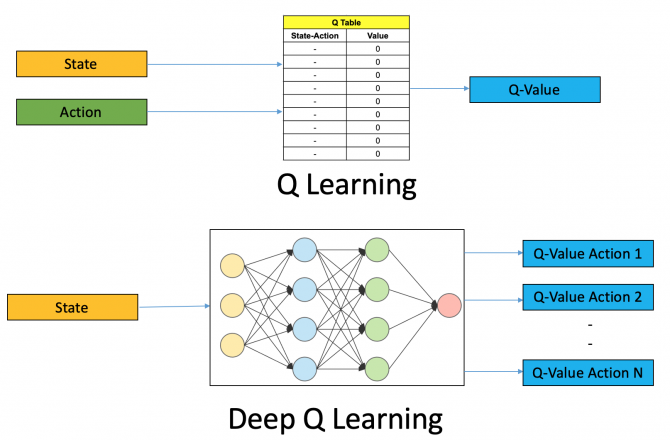
\includegraphics[scale=0.6]{../ReinforcementLearning/fig/deep-q-learning.png}
    \caption{Q-learning vs Deep Q-learning.(Image citation: https://www.mlq.ai/deep-reinforcement-learning-q-learning/)}
    \label{fig:my_label}
\end{figure}\\
While there are several specific variants depending on the problem that is trying to be solved, the general loss function that the neural network tries to minimize at iteration $i$ is as follows:
\begin{equation}
    \mathcal{L}(w_i) = E[(r + \gamma\max_{a'}Q(s', a'; w_{i-1}) - Q(s, a; w_i))^2]
\end{equation}

Here, $(s, a, r, s', a')$ and $\gamma$ are defined the same as in regular Q-learning. $w_i$ are the parameters that the neural net is training during the current iteration of the RL algorithm, and $w_{i-1}$ are the optimal parameters from the previous iteration of the algorithm. The TD error is the term $r + \gamma\max_{a'}Q(s', a';w_{i-1})$, and the squared term inside the expectation is the TD target. Since directly optimizing the loss in equation 12.5 is difficult, gradient descent, specifically stochastic gradient descent is used (in order to avoid having to calculate the entire expected value term in 12.5).\\

The Atari deep Q network that solved the game of brickbreaker used a technique called \textit{experience replay} to make updates to the network more stable. The experience $(s, a, r, s')$ was put into a \textit{replay buffer} which was sampled from to perform minibatch gradient descent to minimize the loss function.
\subsection{Policy Learning}
There are a few situations in which the RL techniques described thus far don't work well or work relatively less well than alternatives:
\begin{enumerate}
    \item The Q function is far more complex than the policy being learned.
    \item The action space is continuous.
    \item Expert knowledge needs to be introduced.
\end{enumerate}
This presents the need for another model-free method called \textbf{policy learning} in which we adopt a differentiable policy $\pi_\theta(a|s)$ parametrized by $\theta$, and try to learn $\theta$ directly without going through a Q function first.\\
We update $\theta$ iteratively according to the following equation:
\begin{equation*}
    \theta \leftarrow \theta + \alpha_t \nabla_\theta J(\theta)
\end{equation*}
where $J(\theta) = E[r(h)]$, $r(h) = \sum_tr_t$, and $h = (s, a, r, s', a', r', s'', a''...)$. The gradient term approximates the performance $V^{\pi}$. We define the likelihood $\mu_\theta(h) = \prod_t\pi_\theta(a_t|s_t)p(s_{t+1}|s_t, a)$. We can expand $\nabla_\theta(\theta)$ as follows:
\begin{equation}
    \nabla_\theta J(\theta) = \nabla_\theta E[r(n)] = \nabla_\theta\int_h\mu_\theta(h)r(h)\delta h = \int_hr(h)\nabla_\theta\mu_\theta(h)\delta h
\end{equation}
We seem to have run into an issue here. The term $\nabla_\theta\mu_\theta(h)$ depends on the transition probability $p(*|s, a)$ by definition, but point of policy learning was to avoid having to learn these transition probabilities. However, it turns out we can circumvent this issue by applying the useful identity
\begin{equation}
    \nabla_\theta\mu_\theta = \mu_\theta\frac{1}{\mu_\theta}\nabla_\theta\mu_\theta = \mu_\theta\nabla_\theta\ln\mu_\theta
\end{equation}
Thus, we can rewrite the previous equation as follows:
\begin{align}
    \int_hr(h)\mu_\theta(h)\nabla_\theta\left[\sum_t\ln\pi_\theta(a_t|s_t) + \sum_t\ln p(s_{t+1}|s_t, a)\right]\delta h\\
    = E\left[r(h)\sum_t\nabla_\theta\ln\pi_\theta(a_t|s_t)\right]\\
    = E\left[\sum_t\nabla_\theta\ln\pi_\theta(a_t|s_t)r_t\right]
\end{align}
Equation 12.10 only involves $\pi_\theta(a_t|s_t)$ which we are trying to learn, and $r_t$ which we observe from the environment. We can now perform SGD to find the optimal $\theta$. Note policy learning is on-policy.
\section{Model-Based Learning}
\begin{figure}[ht!]
    \centering
    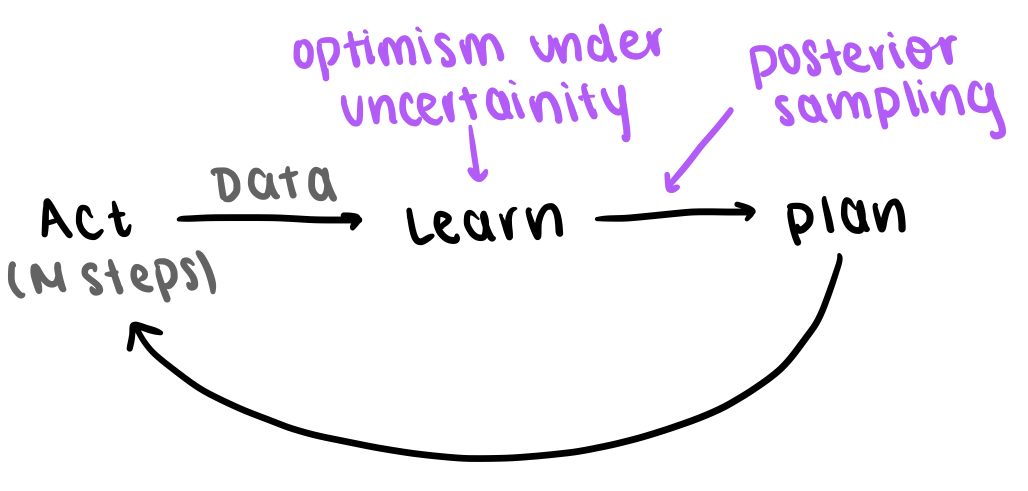
\includegraphics[scale=0.2]{../ReinforcementLearning/fig/model-based.jpeg}
    \caption{The process of model-based learning.}
\end{figure}

\noindent Recall that in model-based learning, the learner tries to learn the parameters of the MDP underlying their environment and then uses planning to come up with a policy. A model-based learner repeats the following three steps until satisfactory performance is achieved:
\begin{enumerate}
    \item Act according to some policy for $M$ steps.
    \item Learn/update a model of the underlying MDP based on the experiences gained from step 1.
    \item Use the model from step 2 to plan for the next $M$ steps.
\end{enumerate}
In many implementations, ``learning" a model means coming up with a maximum likelihood estimate of the parameters of the underlying MDP: the reward function and transition probabilities (we will not cover the specifics of this process in this section). We can now plan according to this model and follow the recommended policy for the next $M$ steps. One issue with this basic model is that it doesn't do anything to handle time spent exploring vs exploiting. While there are many ways to address this in practice, we will now present three common approaches:
\begin{itemize}
    \item Incorporate exploration directly into the policy, for example, by using an $\epsilon$-greedy strategy as discussed in 12.3.1.
    \item \textbf{Optimism under uncertainty}: Let $N(s,a)$ be the number of times we visited the state-action pair $(s,a)$. Each ``visit” is a time that the agent was in state $s$ and chose to perform action $a$. When we are learning, we will assume that if $N(s,a)$ is small, then the next state will have higher reward than predicted by the maximum likelihood model. Since the model thinks taking visiting lesser-known state-action pairs will lead to high reward (we are \textit{optimistic} when we are \textit{uncertain}), we’ll have a tendency to explore these lesser-known areas.
    \item \textbf{Posterior sampling/Thompson sampling}: We maintain a posterior distribution such as a Dirichlet over the transition function $p(*|s, a)$ $\forall s, a$ which we update using the experiences from the previous $M$ steps of acting rather than coming up with a maximum likelihood point estimate. We then \textit{sample} from this posterior to get a model, which we proceed to plan with. The idea is that when we are less certain about the outcome of the transition function, there’s a greater likelihood of the sampling leading us to explore. When we are more certain about what the best outcome is, we’re more likely to just stick with that best outcome.
\end{itemize}
\section{Conclusion}
To recap, reinforcement learning is a machine learning technique that allows a learner to find an optimal policy in an environment modeled by an MDP where the transition probabilities and reward function are unknown. The learner gains information by interacting with the environment and receiving rewards and uses this information to update the model they have of the underlying MDP (model-based) or their beliefs about the value of taking particular actions from particular states (value-based model-free). Q-learning and temporal difference updating are key topics in model-free learning that underlie many techniques in the area including SARSA, Q-learning and deep Q-learning. Contemporary RL models such as the one used by AlphaGo often use a combination of supervised and reinforcement learning methods which can be endlessly customized to meet the needs of a problem.